%%%%%%%%%%%%%%%%%%%%%%%%%%%%%%%%%%%%%%%%%%%%%%%%%%%%%%%%%%%%%%%%%%%%%%%%%%%%%%%
%%
%% Copyright © 2022 Tropic Square s.r.o. (https://tropicsquare.com/)
%%
%% This work is subject to the license terms of the LICENSE.txt file in the
%% root directory of this source tree.
%%
%% If a copy of the LICENSE file was not distributed with this work, you can
%% obtain one at (https://tropicsquare.com/license).
%%
%%%%%%%%%%%%%%%%%%%%%%%%%%%%%%%%%%%%%%%%%%%%%%%%%%%%%%%%%%%%%%%%%%%%%%%%%%%%%%%
%
% This is SPECT programmers manual
%
%%%%%%%%%%%%%%%%%%%%%%%%%%%%%%%%%%%%%%%%%%%%%%%%%%%%%%%%%%%%%%%%%%%%%%%%%%%%%%%

% Specify Tropic Square document class
\documentclass{tropic_design_spec}

\usepackage{listings}
\lstset{backgroundcolor=\color{lightgray}}

%%%%%%%%%%%%%%%%%%%%%%%%%%%%%%%%%%%%%%%%%%%%%%%%%%%%%%%%%%%%%%%%%%%%%%%%%%%%%%%
% Document properties and title page
%%%%%%%%%%%%%%%%%%%%%%%%%%%%%%%%%%%%%%%%%%%%%%%%%%%%%%%%%%%%%%%%%%%%%%%%%%%%%%%
\title{SPECT - Programmers Guide}
\author{Ondrej Ille, Tropic Square}
\date{October 2022}

% Start of document
\begin{document}

% Parameters Needed by Design spec class (must be inside document)
% Set these parameters according to your project.
\def \projectname {SPECT}
\def \documentname {Programmers Guide}
\def \versionnumber {0.5}

% Title page
\maketitle

\newcommand{\tspar}{\par\vspace{0.5cm}}
\newcommand{\tsspc}{\vspace{0.5cm}}
\newcommand{\tsblank}{\hspace*{0.5cm}}
\newcommand{\bi}[1]{\textbf{\textit{#1}}}

\newcommand{\tsnlind}{\newline\tsblank}

\newcommand{\tsif}{\textbf{\textit{if }}}
\newcommand{\tsthen}{\textbf{\textit{then: }}}
\newcommand{\tselse}{\newline\textbf{\textit{else: }}}


%%%%%%%%%%%%%%%%%%%%%%%%%%%%%%%%%%%%%%%%%%%%%%%%%%%%%%%%%%%%%%%%%%%%%%%%%%%%%%%
% Document revisions
%%%%%%%%%%%%%%%%%%%%%%%%%%%%%%%%%%%%%%%%%%%%%%%%%%%%%%%%%%%%%%%%%%%%%%%%%%%%%%%
\section*{Version history}

\begin{TropicRatioLongTable4Col}
    {0.1}            {0.2}                  {0.3}            {0.4}
    {Version Tag     & Date                 & Author          &    Description                    }
     0.1             & 12.10.2022           & Ondrej Ille     &    Initial version                      \Ttlb
     0.2             & 7.11.2022            & Ondrej Ille     &    Fix semantics of LSR instruction.    \Ttlb
     0.3             & 8.11.2022            & Ondrej Ille     &    Fix SCB semantics.                   \Ttlb
     0.4             & 14.11.2022           & Ondrej Ille     &    Fix semantics of ST instruction (op1 instead of op2).
                                                                   Add note about modular instruction operands. \Ttlb
     0.5             & 23.11.2022           & Ondrej Ille     &    Add description of SW toolchain. \Ttlb
\end{TropicRatioLongTable4Col}


%%%%%%%%%%%%%%%%%%%%%%%%%%%%%%%%%%%%%%%%%%%%%%%%%%%%%%%%%%%%%%%%%%%%%%%%%%%%%%%
% Table of contents
%%%%%%%%%%%%%%%%%%%%%%%%%%%%%%%%%%%%%%%%%%%%%%%%%%%%%%%%%%%%%%%%%%%%%%%%%%%%%%%
\pagebreak
\tableofcontents


%%%%%%%%%%%%%%%%%%%%%%%%%%%%%%%%%%%%%%%%%%%%%%%%%%%%%%%%%%%%%%%%%%%%%%%%%%%%%%%
%%%%%%%%%%%%%%%%%%%%%%%%%%%%%%%%%%%%%%%%%%%%%%%%%%%%%%%%%%%%%%%%%%%%%%%%%%%%%%%
% Document
%%%%%%%%%%%%%%%%%%%%%%%%%%%%%%%%%%%%%%%%%%%%%%%%%%%%%%%%%%%%%%%%%%%%%%%%%%%%%%%
%%%%%%%%%%%%%%%%%%%%%%%%%%%%%%%%%%%%%%%%%%%%%%%%%%%%%%%%%%%%%%%%%%%%%%%%%%%%%%%

%%%%%%%%%%%%%%%%%%%%%%%%%%%%%%%%%%%%%%%%%%%%%%%%%%%%%%%%%%%%%%%%%%%%%%%%%%%%%%%
% Glossary
%%%%%%%%%%%%%%%%%%%%%%%%%%%%%%%%%%%%%%%%%%%%%%%%%%%%%%%%%%%%%%%%%%%%%%%%%%%%%%%
\TsSection{Glossary}

\begin{itemize}
    \item{\textbf{CPU} - Central Processing Unit}
    \item{\textbf{ECC} - Eliptic Curve Cryptography}
    \item{\textbf{SPECT} - Secure Processor of Eliptic Curves for Tropic}
\end{itemize}

%%%%%%%%%%%%%%%%%%%%%%%%%%%%%%%%%%%%%%%%%%%%%%%%%%%%%%%%%%%%%%%%%%%%%%%%%%%%%%%
% Register field types
%%%%%%%%%%%%%%%%%%%%%%%%%%%%%%%%%%%%%%%%%%%%%%%%%%%%%%%%%%%%%%%%%%%%%%%%%%%%%%%
\TsSection{Register field types}

\TropicRegisterTypeList


%%%%%%%%%%%%%%%%%%%%%%%%%%%%%%%%%%%%%%%%%%%%%%%%%%%%%%%%%%%%%%%%%%%%%%%%%%%%%%%
% Introduction
%%%%%%%%%%%%%%%%%%%%%%%%%%%%%%%%%%%%%%%%%%%%%%%%%%%%%%%%%%%%%%%%%%%%%%%%%%%%%%%
\TsSection{Introduction}

This document provides a programmer's guide for SPECT. SPECT is a domain specific
processing unit targeted for calculations of Elliptic Curve Cryptography (ECC).
SPECT provides instructions for calculation with 256 bit numbers and modular
arithmetics. SPECT is useful to implement operations/algorithms such as:
\begin{itemize}
    \item{ECDSA - Elliptic Curve Digital Signature Algorithm}
    \item{ECDH  - Elliptic Curve Diffe-Hellman}
\end{itemize}

\begin{figure}[h!]
    \centering
    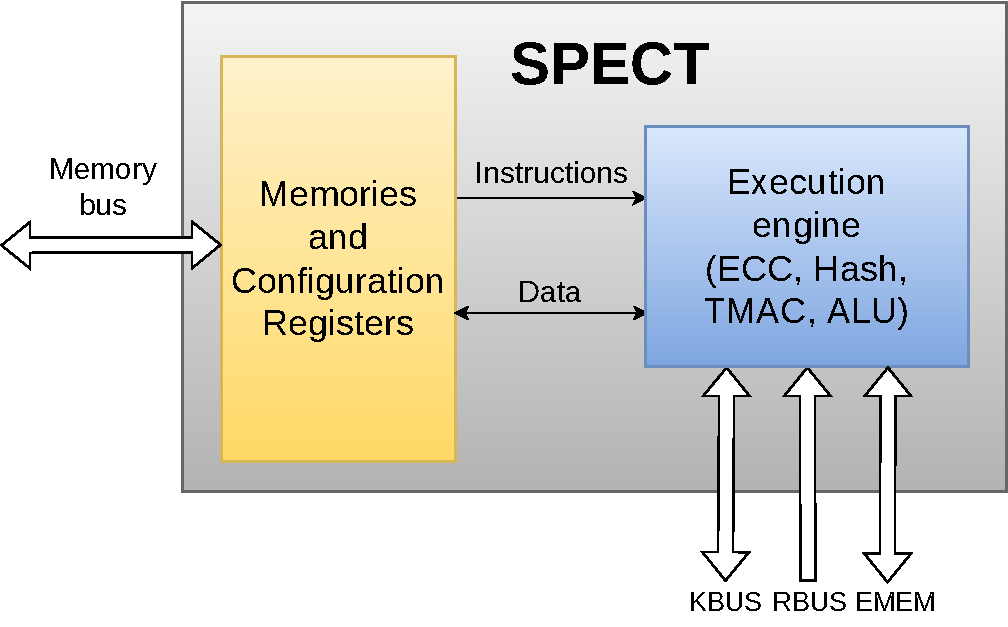
\includegraphics[width=\textwidth,height=\textheight,keepaspectratio]{%
        \detokenize{img/spect_pm_block_diagram.pdf}%
    }
    \caption{SPECT - Block diagram}%
    \label{SPECTBK}%
\end{figure}

\TsSection{Programmer's model}

SPECT programmer's model consists of:
\begin{itemize}
    \item 32 x 256 bit general purpose registers (\textbf{R0} - \textbf{R31}).
    \item \textbf{PC} - Program counter.
    \item Zero (\textbf{Z}) and Carry (\textbf{C}) flag.
    \item HW \textbf{RAR} (Return Address Register) stack for nested procedure calls.
    \item \textbf{SRR} (Secret Results Register) for handling secret results.
    \item 2048 B read-write memory space in address range 0x0000 -- 0x07FC.
    \item 512 B write-only memory space in address range 0x1000 -- 0x11FC.
    \item 2048 B read-only memory space in address range 0x3000 -- 0x37FC.
\end{itemize}

\TropicNote{
    SPECTs address space is 32 bit word organized. \textbf{LD} and \textbf{ST}
    instructions works with 256 bit values and it always uses 8 consecutive words
    in the memory. E.g. 0x0020 - 0x003C.
}

\begin{figure}[h!]
    \centering
    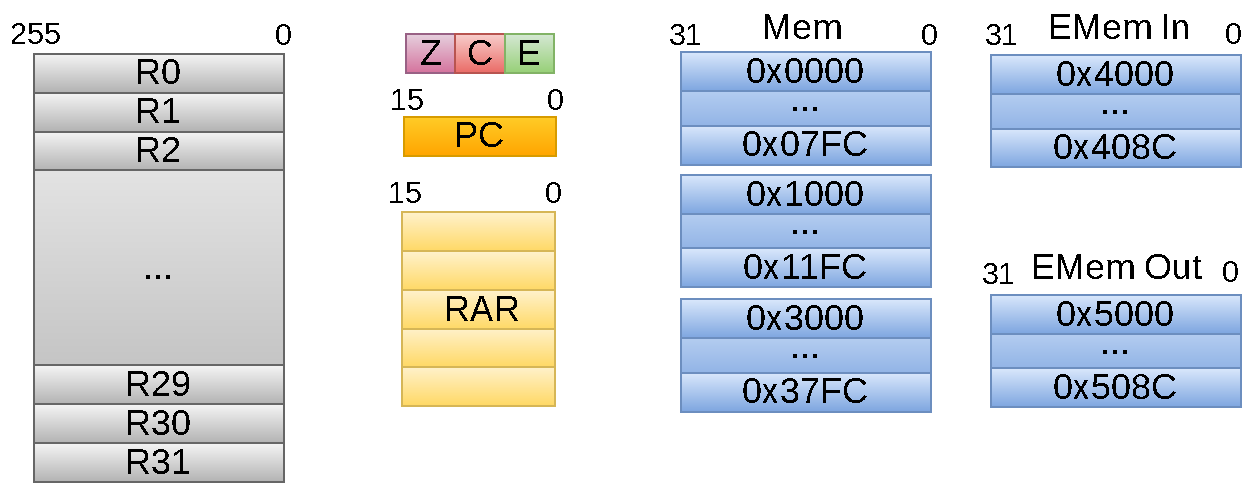
\includegraphics[width=.9\textwidth]{%
        \detokenize{img/spect_pm_gprs.pdf}%
    }
    \caption{SPECT - Programmers model}%
    \label{SPECTBK}%
\end{figure}


\TsSubSection{Subroutine calls}

SPECT contains HW \textbf{RAR} stack, and it pushes return address from subroutine
to RAR stack each time when it executes CALL instruction. When SPECT executes
RET instruction, it pops value from RAR stack and updates \textbf{PC}. HW \textbf{RAR}
stack supports up to 5 nested subroutine calls.

\TropicNote{
    Behavior of SPECT when number of nested subroutine calls is exceeded is undefined.
}

\TsSubSection{Using private keys}

Private keys are typically sensitive information in cryptographic systems.
Therefore, it is good to minimize the time for which they are present in such
system. When SPECT Program needs to use private key which is stored elsewhere
in the system, it executes GPK instruction which reads 256 bit
private key from outside of SPECT. GPK instruction supports key
identification in case of multiple private keys are available in the system.

\TsSubSection{Using random numbers}

Proper random numbers with uniform distribution are critical for cryptographic
calculations. Such random numbers can be typically generated by TRNG (True Random
Number Generator). When SPECT Program needs a random number, it executes GRV
instruction which obtains random number from outside of SPECT.

\TsSubSection{Modular arithmetics}

SPECT provides instructions for finite field arithmetic such as
addition, subtraction and multiplication with 256 bit operands stored in general purpose
registers. SPECT supports fast multiplication in Ed25519 and P-256 curves finite fields 
via dedicated instructions -- MUL25519 and MUL256. Modular arithmetics with generic modulus
specified by value in \textbf{R31} is supported by instructions ADDP, SUBP, MULP. SPECT
also supports modular reduction of 512 bit number with REDP instruction.

When programming with modular instructions, one needs to be careful about input
operands of such instructions. Following conditions must be met:
\begin{itemize}
    \item op2 < $P_{25519}$ and op3 < $P_{25519}$ for MUL25519 instruction.
    \item op2 < $P_{256}$ and op3 < $P_{256}$ for MUL256 instruction.
    \item op2 < R31 and op3 < R31 for ADDP, SUBP instructions.
    \item R31 != 0 and R31 != 1 for ADDP, SUBP, MULP, REDP instructions.
\end{itemize}
if these conditions are not met when invoking such modular instruction, result
of instruction calculation is undefined (value in op1).

\TropicNote{
    Performance of MULP when \textbf{R31} = $P_{25519}$ / $P_{256}$ is lower
    than performance of MUL25519 / MUL256.
}

\TsSubSection{Hash calculation}

SPECT supports SHA512 Hash calculation as specified in FIPS 180-4. SPECT can
calculate SHA512 hash from arbitrarily long data stream. When SPECT executes HASH_IT
instruction, it resets context in its execution engine to initialization
vector as specified in FIPS 180-4. Each execution of HASH instruction
processes 1024 bit block, and executes next round of SHA512 calculation.

\TropicNote{
    SPECT does not perform padding of input data as specified in section 5.1
    of FIPS 180-4. It is responsibility of SPECT program or external system
    to perform such padding.
}

\TsSubSection{Handling secret results}

Cryptographic calculations frequently result in a shared secret (e.g. in case
of ECDH calculation), which shall only be visible to certain other objects in
the system, but it shall not be globally accessible on system level memory bus.
When SPECT program finishes its execution, it stores these results into
\textbf{SRR} register. After the program execution has finished, external
blocks within a system can read this secret result from the SPECT via dedicated
handshake.

\TsSubSection{Scalar blinding}

SPECT supports scalar blinding by a random number as side-channel counter-measure
by SCB instruction. It blinds the scalar $sc$ using group scalar randomization method
as defined in \cite{SCB} with 256 bit random number. The random number $rng$ shall be obtained in
advance by GRV instruction as described above. The group order $q$ shall be present in \textbf{R31}.

SCB performs this exact function: $$Blind(sc, rng, q) = q \times (rng | (2^{255} + 2^{223})) + sc$$

\TsSubSection{SPECT invocation}

SPECT is invoked by external system which has access to its memory space via
memory bus as shown in following figure:

\begin{figure}[h!]
    \centering
    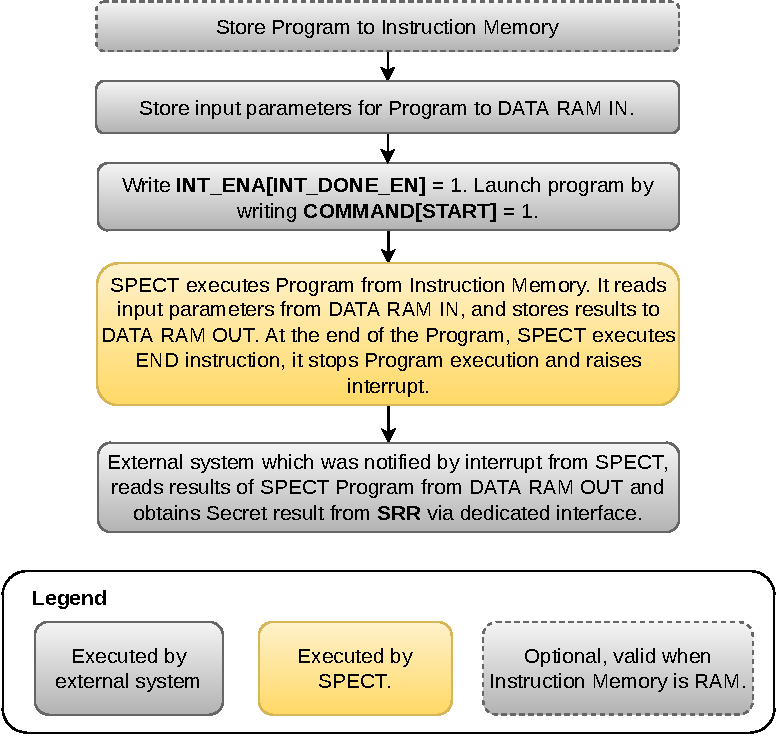
\includegraphics[width=.7\textwidth]{%
        \detokenize{img/spect_pm_invocation.pdf}%
    }
    \caption{SPECT - Invocation}%
    \label{SPECTBK}%
\end{figure}

\TropicNote{Address of first Program instruction executed by SPECT after
            \Register{COMMAND[START]} = 1 is written, is fixed and defined
            by a system which integrates SPECT.}

\TsSubSection{Invalid instructions}

When SPECT attempts to execute invalid instruction, it aborts program execution
and sets \Register{STATUS[ERR]} = 1.

\TropicNote{
    Invalid instruction means invalid opcode or not matching parity bit in the instruction code. Unless
    a fault, usual cause of this is e.g. missing RET instruction in subroutine or END instruction at the
    end of program.
}

\TsSubSection{Soft Reset}

SPECT can be reset by extenal system by writing \Register{COMMAND[RST]} = 1.
When SPECT is reset, it aborts program execution and resets its internal state.

\TsSubSection{Interrupts}

SPECT program execution can't be interrupted by an external event (other than
Soft reset). SPECT itself can generate following interrupts for external system:
\begin{itemize}
    \item{Program Done - Enabled when \Register{INT_ENA[INT_DONE_EN]} = 1. Generated
                         when SPECT program executes END instruction, or it
                         detects error.}
    \item{Program Error interrupt - Enabled when \Register{INT_ENA[INT_DONE_EN]} = 1.
                        Generated when SPECT attempts to execute invalid instruction.}
\end{itemize}


%%%%%%%%%%%%%%%%%%%%%%%%%%%%%%%%%%%%%%%%%%%%%%%%%%%%%%%%%%%%%%%%%%%%%%%%%%%%%%%
% Instruction set
%%%%%%%%%%%%%%%%%%%%%%%%%%%%%%%%%%%%%%%%%%%%%%%%%%%%%%%%%%%%%%%%%%%%%%%%%%%%%%%

\TsSection{Instruction set}

SPECT provides 4 types of instructions:
\begin{itemize}
    \item{\textbf{R} - Register}
    \item{\textbf{I} - Immediate}
    \item{\textbf{M} - Memory}
    \item{\textbf{J} - Jump}
\end{itemize}

\TsSubSection{Operand interpretation}

All operands are considered as 256 bits unsigneds. Arithmetic instructions working only with 32 bit
operands ignores the 224 MSBs of input and clears them in the result. Logic instructions
working only with 32 bit operands also ignores the 224 MSBs of input, but passes the 224 MSBs of op2
to the result.

\TsSubSection{Instruction Format}

\definecolor{instgray}{RGB}{235, 235, 235}
    \begin{table}[h]
        \begin{center}
            \setlength{\tabcolsep}{4pt}
            \small
            \begin{tabular}{c c c c c c c c c c c c c c c c c c c c c c c c c c c c c c c c l}
            31 & 30 & 29 & 28 &
               &    & 25 & 24 &
               & 22 & 21 &    &
               &    & 17 & 16 &
            15 &    &    & 12 &
            11 &    &    &    &
            07 & 06 &    &    &
               &    &    & 00 & \\
            \hline
            \multicolumn{1}{|c|}{p} &
            \multicolumn{2}{c|}{\cellcolor{instgray}type} &
            \multicolumn{4}{c|}{\cellcolor{instgray}opcode} &
            \multicolumn{3}{c|}{\cellcolor{instgray}func} &
            \multicolumn{5}{c|}{\cellcolor{instgray}op1} &
            \multicolumn{5}{c|}{\cellcolor{instgray}op2} &
            \multicolumn{5}{c|}{\cellcolor{instgray}op3} &
            \multicolumn{7}{c|}{} &
            \textbf{R}\\
            \hline
            \\
            \hline
            \multicolumn{1}{|c|}{p} &
            \multicolumn{2}{c|}{\cellcolor{instgray}type} &
            \multicolumn{4}{c|}{\cellcolor{instgray}opcode} &
            \multicolumn{3}{c|}{\cellcolor{instgray}func} &
            \multicolumn{5}{c|}{\cellcolor{instgray}op1} &
            \multicolumn{5}{c|}{\cellcolor{instgray}op2} &
            \multicolumn{12}{c|}{\cellcolor{instgray}Immediate} &
            \textbf{I}\\
            \hline
            \\
            \hline
            \multicolumn{1}{|c|}{p} &
            \multicolumn{2}{c|}{\cellcolor{instgray}type} &
            \multicolumn{4}{c|}{\cellcolor{instgray}opcode} &
            \multicolumn{3}{c|}{\cellcolor{instgray}func} &
            \multicolumn{5}{c|}{\cellcolor{instgray}op1} &
            \multicolumn{1}{c|}{} &
            \multicolumn{16}{c|}{\cellcolor{instgray}Addr} &
            \textbf{M}\\
            \hline
            \\
            \hline
            \multicolumn{1}{|c|}{p} &
            \multicolumn{2}{c|}{\cellcolor{instgray}type} &
            \multicolumn{4}{c|}{\cellcolor{instgray}opcode} &
            \multicolumn{3}{c|}{\cellcolor{instgray}func} &
            \multicolumn{6}{c|}{} &
            \multicolumn{16}{c|}{\cellcolor{instgray}NewPC} &
            \textbf{J}\\
            \hline
            \end{tabular}
        \end{center}
        %\caption{Instruction Format}
    \end{table}

\TsSubSection{Symbols}

Following symbols are used in description of instructions:
\begin{itemize}
    \item{|| -- Bitwise concatenation}
    \item{$P_{25519} = 2^{255} - 19$}
    \item{$P_{256} = 2^{256} - 2^{224} + 2^{192} + 2^{96} - 1$}
    \item{F -- Flags set by the instruction}
    \item{\#C -- Number of cycles the instruction takes to execute}
\end{itemize}


\begin{landscape}
\pagebreak
\TsSubSection{R instructions}
\begin{TropicRatioLongTable5Col}
    {0.25}                   {0.285}                              {0.4}                                   {0.03} {0.035}
    {Mnemonic               & Name                              & Semantics                             & F      & \#C              }
      \TropicTableBreak{32 bit arithmetic instructions}                                                                             \Ttlb
      ADD op1,op2,op3       & 32 bit adition                    & op1 = op2 + op3                       & Z      & 11               \Ttlb
      SUB op1,op2,op3       & 32 bit subtraction                & op1 = op2 - op3                       & Z      & 11               \Ttlb
      CMP op2,op3           & 32 bit comparison                 & op2 - op3                             & Z      & 9                \Ttlb

      \TropicTableBreak{32 bit logic instructions}                                                                                  \Ttlb
      AND op1,op2,op3       & 32 bit bitwise AND                & op1 = op2 \& op3                      & Z      & 11               \Ttlb
      OR op1,op2,op3        & 32 bit bitwise OR                 & op1 = op2 | op3                       & Z      & 11               \Ttlb
      XOR op1,op2,op3       & 32 bit bitwise Exclusive OR       & op1 = op2 \textasciicircum\space op3  & Z      & 11               \Ttlb
      NOT op1,op2           & 32 bit bitwise NOT                & op1 = \textasciitilde op2             & Z      & 10               \Ttlb

      \TropicTableBreak{Shift Instructions}                                                                                         \Ttlb
      LSL op1,op2           & Logic shift left                  & op1 = op2[254:0] || 0                 & C      & 10               \Ttlb
      LSR op1,op2           & Logic shift right                 & op1 = 0 || op2[255:1]                 & C      & 10               \Ttlb
      ROL op1,op2           & Rotating shift left               & op1 = op2[254:0] || op2[255]          & C      & 10               \Ttlb
      ROR op1,op2           & Rotating shift right              & op1 = op2[0] || op2[255:1]            & C      & 10               \Ttlb
      ROL8 op1,op2          & Rotating byte shift left          & op1 = op2[247:0] || op2[255:248]      &        & 10               \Ttlb
      ROR8 op1,op2          & Rotating byte shift right         & op1 = op2[7:0] || op2[255:8]          &        & 10               \Ttlb
      SWE op1,op2           & Swap endianity                    & op1[255:248] = op2[7:0]  \newline
                                                                  op1[247:240] = op2[15:8] \newline
                                                                  ... \newline
                                                                  op1[7:0] = op2[255:248]               &        & 10               \Ttlb

      \TropicTableBreak{Modular arithmetic instructions}                                                                            \Ttlb
      MUL25519 op1,op2,op3  & Multiplication in $GF(P_{25519})$ & op1 = (op2 * op3) \% $P_{25519}$      &        & 91               \Ttlb
      MUL256 op1,op2,op3    & Multiplication in $GF(P_{256})$   & op1 = (op2 * op3) \% $P_{256}$        &        & 139              \Ttlb
      ADDP op1,op2,op3      & Generic Modular Addition          & op1 = (op2 + op3) \% R31              &        & 16               \Ttlb
      SUBP op1,op2,op3      & Generic Modular Subtraction       & op1 = (op2 - op3) \% R31              &        & 16               \Ttlb
      MULP op1,op2,op3      & Generic Modular Multiplication    & op1 = (op2 * op3) \% R31              &        & 597              \Ttlb
      REDP op1,op2,op3      & Generic Modular Reduction         & op1 = (op2 || op3) \% R31             &        & 528              \Ttlb

      \TropicTableBreak{Other Instructions}                                                                                         \Ttlb
      MOV op1,op2           & Move register                     & op1 = op2                             &        & 7                \Ttlb
      CSWAP op1,op2         & Conditional swap                  & \tsif \textbf{C} == 1 \tsthen \tsnlind
                                                                    op1 = op2 \tsnlind
                                                                    op2 = op1                           &        & 11               \Ttlb
      HASH op1,op2          & Hash                              & tmp = \textit{SHA512}(op2+3||op2+2||op2+1||op2)\newline
                                                                  op1 = tmp[255:0]\newline
                                                                  op1+1 = tmp[511:256]                  &        & 347              \Ttlb
      GRV op1               & Get Random Value                  & op1 = Random number                   &        &  --              \Ttlb
      SCB op1,op2,op3       & Blind scalar                      & B = \textit{Blind}(op2, op3, R31)\newline
                                                                  op1 = B[255:0]\newline
                                                                  op1+1 = B[511:256]                    &        & 88               \Ttlb
\end{TropicRatioLongTable5Col}


\TsSubSection{I instructions}
\begin{TropicRatioLongTable5Col}
    {0.25}                      {0.285}                              {0.4}                                          {0.03} {0.035}
    {Mnemonic                   & Name                              & Semantics                                     & F      & \#C          }
      \TropicTableBreak{32 bit arithmetic instructions}                                                                                     \Ttlb
      ADDI op1,op2,Immediate    & 32 bit addition                   & op1 = op2 + Immediate                         & Z     & 11            \Ttlb
      SUBI op1,op2,Immediate    & 32 bit subtraction                & op1 = op2 - Immediate                         & Z     & 11            \Ttlb
      CMPI op2,Immediate        & 32 bit comparison                 & op2 - Immediate                               & Z     & 9             \Ttlb

      \TropicTableBreak{12 bit logic instructions}                                                                                          \Ttlb
      ANDI op1,op2,Immediate    & 12 bit bitwise logic AND          & op1 = op2 \& Immediate                        & Z     & 11            \Ttlb
      ORI op1,op2,Immediate     & 12 bit bitwise logic OR           & op1 = op2 | Immediate                         & Z     & 11            \Ttlb
      XORI op1,op2,Immediate    & 12 bit bitwise exclusive OR       & op1 = op2 \textasciicircum\space Immediate    & Z     & 11            \Ttlb
      \TropicTableBreak{Other Instructions}                                                                                                 \Ttlb
      CMPA op2,Immediate        & comparison                        & \tsif op2 == Immediate \tsthen \tsnlind
                                                                        Z = 1
                                                                      \tselse\tsnlind
                                                                        Z = 0                                       & Z     & 9             \Ttlb

      MOVI op1,Immediate        & Move immediate                    & op1[11:0] = Immediate,\newline
                                                                      op1[255:12] = 0                               &       & 6             \Ttlb
      HASH_IT                   & Hash init                         & Reset hash calculation.                       &       & 9             \Ttlb
      GPK op1, Immediate        & Get Private Key                   & op1 = Private key, Key index = immediate      &       & --            \Ttlb
\end{TropicRatioLongTable5Col}

Due to not enought space in the 32 bit instruction format, the immediate operand is just 12 bit. Because of that,
the logic instructions works only with the 12 LSBs of op2. E.g. 0xFF12 \& 0xF0F = 0xFF02.

\TsSubSection{M instructions}

\begin{TropicRatioLongTable5Col}
    {0.25}                      {0.285}                            {0.4}                                           {0.03}  {0.035}
    {Mnemonic                   & Name                              & Semantics                                     & F     & \#C                   }
      LD op1,Addr               & Load                              & op1[31:0] = Mem[Addr]\newline
                                                                      op1[63:32] = Mem[Addr+0x4]\newline
                                                                      ...\newline
                                                                      op1[255:224] = Mem[Addr+0x1C]                 &       & 21            \Ttlb
      ST op2,Addr               & Store                             & Mem[Addr] = op1[31:0]\newline
                                                                      Mem[Addr+0x4] = op1[63:32] = \newline
                                                                      ...\newline
                                                                      Mem[Addr+0x1C] = op1[255:224]                 &       & 12            \Ttlb
\end{TropicRatioLongTable5Col}

\pagebreak
\TsSubSection{J instructions}

\begin{TropicRatioLongTable5Col}
    {0.25}                      {0.285}                             {0.4}                                           {0.03}  {0.035}
    {Mnemonic                   & Name                              & Semantics                                     & F      & \#C           }
     CALL NewPC                 & Subroutine call                   & push(RAR, PC+0x4), PC = NewPC                 &        & 5            \Ttlb
     RET                        & Return from subroutine            & PC = pop(RAR)                                 &        & 5            \Ttlb
     BRZ NewPC                  & Branch on Zero                    & \tsif Z == 1 \tsthen \tsnlind
                                                                        PC = NewPC                                  &        & 5            \Ttlb
     BRNZ NewPC                 & Branch on not Zero                & \tsif Z == 0 \tsthen \tsnlind
                                                                        PC = NewPC                                  &        & 5            \Ttlb
     BRC NewPC                  & Branch on Carry                   & \tsif C == 1 \tsthen \tsnlind
                                                                        PC = NewPC                                  &        & 5            \Ttlb
     BRNC NewPC                 & Branch on not Carry               & \tsif C == 0 \tsthen \tsnlind
                                                                        PC = NewPC                                  &        & 5            \Ttlb
     JMP NewPC                  & Unconditional jump                & PC = NewPC                                    &        & 5            \Ttlb
\end{TropicRatioLongTable5Col}

\end{landscape}


%%%%%%%%%%%%%%%%%%%%%%%%%%%%%%%%%%%%%%%%%%%%%%%%%%%%%%%%%%%%%%%%%%%%%
% 
% Autogenerated by TS Memory Map Generator
% Input: /projects/tropic01/work/vmasek/ts-spect/reg_map/spect_mem_map.yml
% Date: 09:38AM on May 11, 2023
%
%%%%%%%%%%%%%%%%%%%%%%%%%%%%%%%%%%%%%%%%%%%%%%%%%%%%%%%%%%%%%%%%%%%%%
%%%%%%%%%%%%%%%%%%%%%%%%%%%%%%%%%%%%%%%%%%%%%%%%%%%%%%%%%%%%%%%%%%%%%
% SPECT Memory Map
%%%%%%%%%%%%%%%%%%%%%%%%%%%%%%%%%%%%%%%%%%%%%%%%%%%%%%%%%%%%%%%%%%%%%
\pagebreak
\TsSection {SPECT Memory Map}

\textbf{Base Address:} 0x0000 0000
\newline
\textbf{End Address:} 0x0000 9FFF
\vspace{4mm}

\begin{TropicRatioTable3Col}
{0.6}                                         {0.3}                               {0.1}
{Memory region                                & Address offset range              & Size}

        \multirow {2} {*} {\hyperref[subsec:Data RAM IN] {Data RAM IN}} & 0x0000 0000 & \multirow {2} {*} {2 KB} \\
                                                    & 0x0000 07FF &    \Ttlb%
        
        \multirow {2} {*} {\hyperref[subsec:Data RAM OUT] {Data RAM OUT}} & 0x0000 1000 & \multirow {2} {*} {512 bytes} \\
                                                    & 0x0000 11FF &    \Ttlb%
        
        \multirow {2} {*} {\hyperref[subsec:Configuration registers] {Configuration registers}} & 0x0000 2000 & \multirow {2} {*} {16 bytes} \\
                                                    & 0x0000 200F &    \Ttlb%
        
        \multirow {2} {*} {\hyperref[subsec:Constants ROM] {Constants ROM}} & 0x0000 3000 & \multirow {2} {*} {2 KB} \\
                                                    & 0x0000 37FF &    \Ttlb%
        
        \multirow {2} {*} {\hyperref[subsec:External Memory In] {External Memory In}} & 0x0000 4000 & \multirow {2} {*} {64 bytes} \\
                                                    & 0x0000 403F &    \Ttlb%
        
        \multirow {2} {*} {\hyperref[subsec:External Memory Out] {External Memory Out}} & 0x0000 5000 & \multirow {2} {*} {80 bytes} \\
                                                    & 0x0000 504F &    \Ttlb%
        
        \multirow {2} {*} {\hyperref[subsec:Instruction Memory] {Instruction Memory}} & 0x0000 8000 & \multirow {2} {*} {8 KB} \\
                                                    & 0x0000 9FFF &    \Ttlb%
        
\end{TropicRatioTable3Col}

%%%%%%%%%%%%%%%%%%%%%%%%%%%%%%%%%%%%%%%%%%%%%%%%%%%%%%%%%%%%%%%%%%%%%
% Configuration registers
%%%%%%%%%%%%%%%%%%%%%%%%%%%%%%%%%%%%%%%%%%%%%%%%%%%%%%%%%%%%%%%%%%%%%
\pagebreak
\TsSubSection {Configuration registers}

\textbf{Base Address:} 0x0000 2000
\newline
\textbf{End Address:} 0x0000 200F
\vspace{4mm}
%   Ordt 230321.01 autogenerated file 
%   Input: /projects/tropic01/work/vmasek/ts-spect/reg_map/reg_map.rdl
%   Parms: /projects/tropic01/work/vmasek/ts-spect/doc/design_specification/temp_parms_files/reg_map.parms
%   Date: Thu May 11 09:38:24 CEST 2023
%

% Register Summary table
\begin{TropicRatioTable3Col}
{0.15} {0.65} {0.2}
{Address Offset & Register Name & Reset Value}
0x0 & \hyperlink{spect:BLOCK ID}{BLOCK_ID} & 0x000-0030\Ttlb%
0x4 & \hyperlink{spect:COMMAND}{COMMAND} & 0x00000000\Ttlb%
0x8 & \hyperlink{spect:STATUS}{STATUS} & 0x00000001\Ttlb%
0xc & \hyperlink{spect:INT ENA}{INT_ENA} & 0x00000000\Ttlb%
\end{TropicRatioTable3Col}

\pagebreak

\begin{landscape}

{\hypertarget{spect:BLOCK ID}{}}
\begin{TropicRegisterLandscapeTable}
  [Address:]%
  {BLOCK_ID}%
  {0x2000}%
  ID_CODE & RO & 0x30 & 15:0 & Identification code \Ttlb
  REV_CODE & RO & - & 19:16 & Revision code \Ttlb
\end{TropicRegisterLandscapeTable}


{\hypertarget{spect:COMMAND}{}}
\begin{TropicRegisterLandscapeTable}
  [Address:]%
  {COMMAND}%
  {0x2004}%
  START & WO W1S; & 0x0 & 0:0 & Starts SPECT FW operation \Ttlb
  SOFT_RESET & WO & 0x0 & 1:1 & Stops FW execution and resets SPECT \Ttlb
\end{TropicRegisterLandscapeTable}


{\hypertarget{spect:STATUS}{}}
\begin{TropicRegisterLandscapeTable}
  [Address:]%
  {STATUS}%
  {0x2008}%
  IDLE & RO & 0x1 & 0:0 & SPECT is in IDLE mode \Ttlb
  DONE & RW W1C & 0x0 & 1:1 & Active when SPECT successfully completes the calculation \Ttlb
  ERR & RW W1C & 0x0 & 2:2 & Active when SPECT ends the calculation with error \Ttlb
\end{TropicRegisterLandscapeTable}


{\hypertarget{spect:INT ENA}{}}
\begin{TropicRegisterLandscapeTable}
  [Address:]%
  {INT_ENA}%
  {0x200c}%
  INT_DONE_EN & RW & 0x0 & 0:0 & Enables DONE interrupt \Ttlb
  INT_ERR_EN & RW & 0x0 & 1:1 & Enables ERROR interrupt \Ttlb
\end{TropicRegisterLandscapeTable}


\end{landscape}


\TsSubSection{Data RAM IN}

Data RAM IN is a memory where external system stores parameters for SPECT Program
before it starts its execution. SPECT Program sees it as read-write memory.

\TsSubSection{Data RAM OUT}

Data RAM OUT is a memory where SPECT Program stores results of its calculation,
and external system reads such results after SPECT Program execution ends. SPECT
Program sees it as write-only memory.

\TsSubSection{Instruction Memory}

Instruction memory contains the Program executed by SPECT. Based on SPECT
manufacturing configuration, this memory might be readable/writable by external
system (Instruction Memory is RAM), or not accessible by external system at all
(Instruction Memory is ROM with fixed program). SPECT Program do not have access
to this memory with LD and ST instructions. 

\TsSubSection{Constant ROM}

Constant ROM contains a ROM image with important cryptographic constants
used by SPECT Program during program execution. SPECT program sees it as
read-only memory.

\OpenIssue{Place SPECT Constant ROM content!}

%%%%%%%%%%%%%%%%%%%%%%%%%%%%%%%%%%%%%%%%%%%%%%%%%%%%%%%%%%%%%%%%%%%%%%%%%%%%%%%
% SW supoort
%%%%%%%%%%%%%%%%%%%%%%%%%%%%%%%%%%%%%%%%%%%%%%%%%%%%%%%%%%%%%%%%%%%%%%%%%%%%%%%
\TsSection{SW toolchain}

SPECT contains SW toolchain intended for SW development and debugging. SPECT
has following applications available:

\begin{itemize}
    \item{spect_compiler} -- A compiler/assembler which creates .hex file from .s
                            assembly file.
    \item{spect_iss} -- Instruction level simulator with simple command line debugger.
                       It can simulate .s file as well as .hex file.
\end{itemize}

Options for each of the applications are described when using \textbf{- -help}
command line option. Options available inside interactive shell of
\textbf{spect_iss} are available with \textbf{- -help} command line oprion or \textbf{help}
command.

SPECT assembler has support for following assembly language features:
\begin{itemize}
    \item{Function labels}
    \item{Constant definitions}
    \item{Include other assembly file}
\end{itemize}

\TsSubSection{Tool requirements}

SPECT SW toolchain requires following tools:
\begin{itemize}
    \item CMAKE 3.18.2 or higher
\end{itemize}

\OpenIssue{What else?}

\TsSubSection{Function labels}

SPECT compiler allows definition of function labels, and passing them
as NewPc of J instructions, e.g like so:

\begin{lstlisting}
_start:
    CALL my_func
    END

my_func:
    ADD r0, r1, r2
    RET
\end{lstlisting}


\TsSubSection{Constant definitions}
SPECT compiler allows definition of constants, and passing them as
Addr of M instructions or Immediate operand of I type instructions like so:

\begin{lstlisting}
threshold .eq 0x12

_start:
    ADDI r0, r0, threshold
\end{lstlisting}

\begin{lstlisting}
p25519_addr .eq 0x3020

_start:
    LD r31, p25519_addr
\end{lstlisting}

\TropicNote{
    Currently, SPECT compiler does not support expression parsing,
    it only supports simple decimal, hexadecimal or binary value
    when defining constants.
}

\TsSubSection{Include other assembly file}

Multiple .s assembly files can be connected together in SPECT source code
via "include" directive, e.g. like so:

\begin{lstlisting}
_start:
    NOP

.include <other_s_file>
    END
\end{lstlisting}

\section{REFERENCES}\label{s:REFERENCES}

\begin{thebibliography}{99}

    \bibitem{SCB}{
        Danger, Jean-Luc et al.
        “A synthesis of side-channel attacks on elliptic curve cryptography in smart-cards.”
        Journal of Cryptographic Engineering 3 (2013): 241 - 265.
    }

\end{thebibliography}


%%%%%%%%%%%%%%%%%%%%%%%%%%%%%%%%%%%%%%%%%%%%%%%%%%%%%%%%%%%%%%%%%%%%%%%%%%%%%%%
% Open issues
%%%%%%%%%%%%%%%%%%%%%%%%%%%%%%%%%%%%%%%%%%%%%%%%%%%%%%%%%%%%%%%%%%%%%%%%%%%%%%%
\TsSection{Open Issues}

\PrintOpenIssueSummary

\end{document}